% !TEX root = ../main.tex

\chapter{基于分层卷积神经网络的高光谱图像多尺度特征学习与分类}[A Hybrid 3D–2D Feature Hierarchy CNN with Focal Loss for
Hyperspectral Image Classification]

\section{引言}[Introduction]

随着深度学习的不断发展,卷积神经网络(Convolutional Neural Network, CNN)在包括图像分类、实例检测、语义分割等多个图像识别任务中都表现出了颇具竞争力的表现。因此,
作为基于学习的特征提取方法之一,卷积神经网络逐步成为研究高光谱图像分类的关键技术要素。然而,卷积神经网络原生的卷积核设计,导致其只对单一尺度局部感受野内的模式进行构建。
因此,设计多尺度的卷积核学习多级语义,才能应对复杂场景下的高光谱图像分类任务。基于以上应用需求,本章以高光谱图像的光谱和空间特征联合学习为背景,研究基于卷积神经网络的
多尺度语义学习技术,以提升高光谱图像特征的表达能力及地物分类的精度。\par
通常,在标签样本中少部分类的样本数据占据很大的比例,相反地,大部分类只有少量的样本。上述普遍的样本分布规律被称之为长尾数据分布(Long-tailed Data Distribution),是
模型在尾部类分类性能降级的主要原因之一。为此,本章将结合基于卷积神经网络的多尺度语义表示,通过重加权的形式,设计缓解长尾分布分类问题的焦点损失(Focal Loss),调整决策
边界,进一步提高地物分类精度。

\section{混合卷积}[]
% start
毕业论文双语题注如\figref{golfer1}所示。
\lipsum[1]

\begin{figure}[!h]
	\centering
	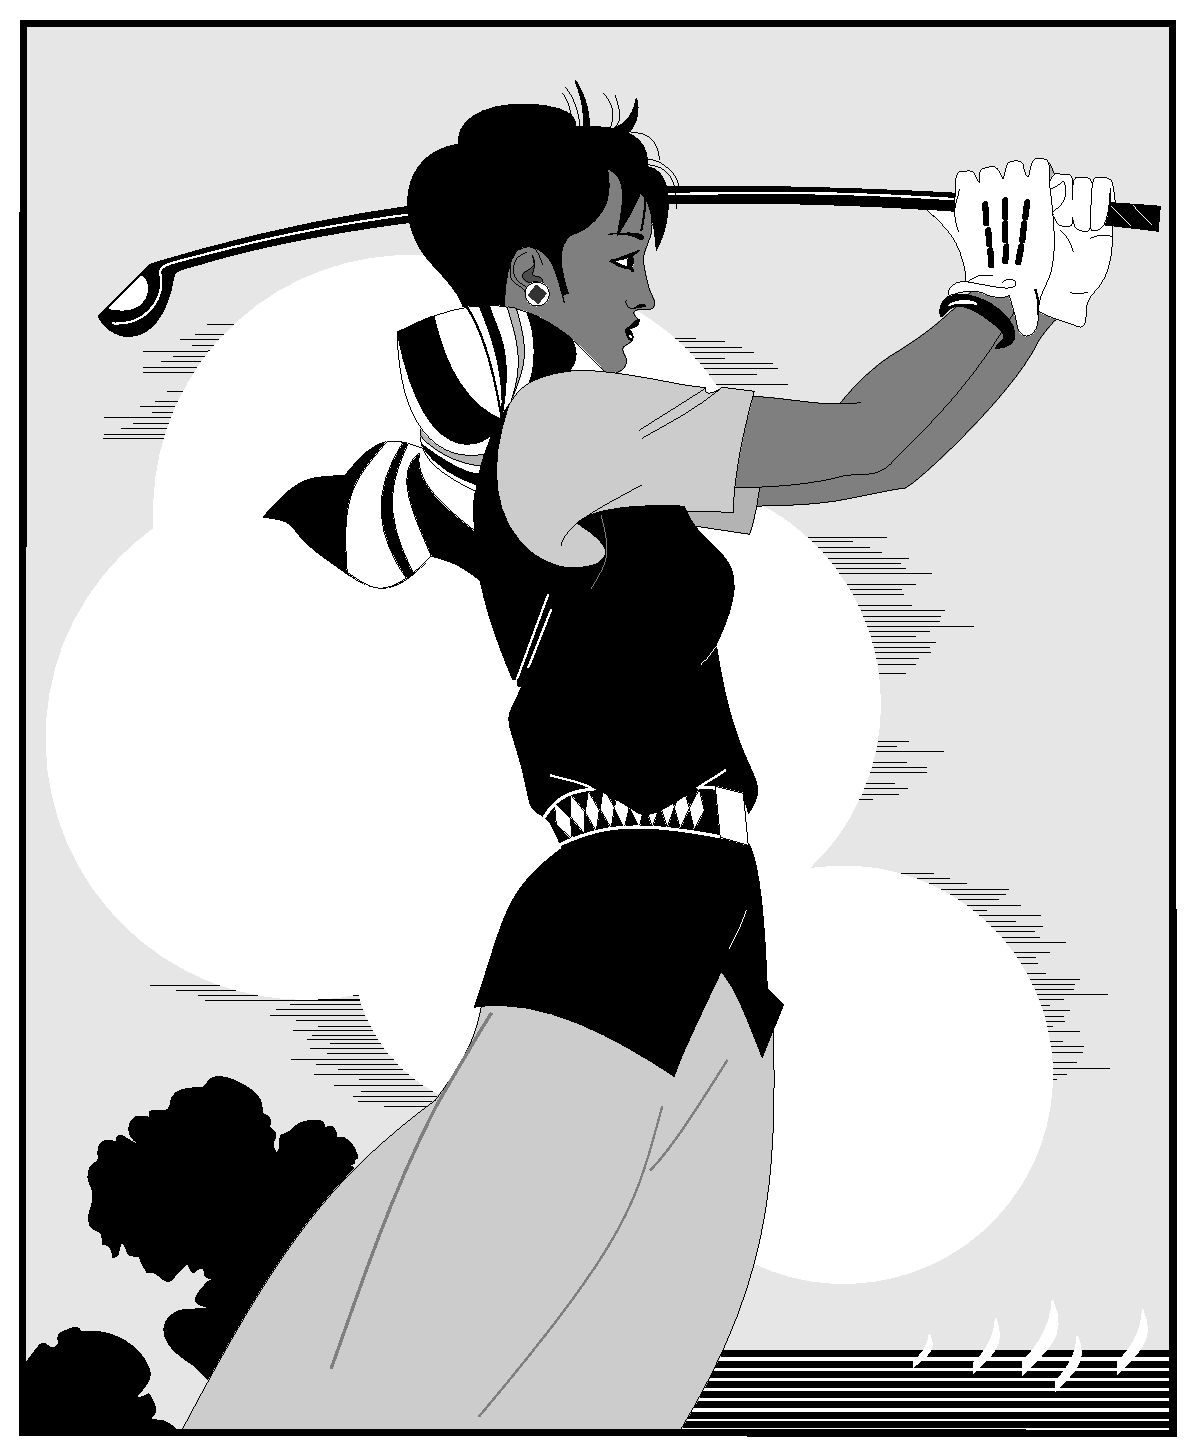
\includegraphics[width = 0.4\textwidth]{golfer}
	\bicaption[golfer1]{}{打高尔夫球球的人(博士论文双语题注)}{Fig.$\!$}{The person playing golf (Doctoral thesis)}
\end{figure}


\section{焦点函数设计}[Design of the Focal loss]
% start
\lipsum[1]


\section{实验结果及分析}[Experimental results and analyses]
% start
\lipsum[1]


\section{本章小结}[Brief summary]
% start
% 随机生成一段文字
\lipsum[1]
